\documentclass[a4paper,11pt]{article}

\usepackage[utf8]{inputenc}
\usepackage{booktabs, array, pdflscape}
\usepackage{geometry}
\usepackage{graphics,subfigure,graphicx}
\usepackage{color}
\usepackage{url}
\usepackage{enumerate}
\usepackage[table]{xcolor}

\pagestyle{headings}

\setlength{\textheight}{24cm}  
\setlength{\textwidth}{15cm}
\setlength\oddsidemargin{0cm}
\setlength\evensidemargin{0cm}
\setlength\voffset{-1cm}

\renewcommand{\textfraction}{0.01}
\renewcommand{\floatpagefraction}{0.75}
\renewcommand{\topfraction}{0.8}
\renewcommand{\bottomfraction}{0.8}

\newcommand{\red}[1]{\textcolor{red}{#1}}	
\newcommand{\mc}[3]{\multicolumn{#1}{#2}{#3}}

\newcommand{\Ni}{({\em i\,})~}
\newcommand{\Nii}{({\em ii\,})~}
\newcommand{\Niii}{({\em iii\,})~}

%opening
\title{

\includegraphics[width=3cm]{./img/200px-SuitClubs.png} \\
\Huge Evaluation plan for CLUBS project \\ 
}
\author{\vspace*{1cm}\\ \LARGE Juliane Stiller \& Vivien Petras \medskip \\ \Large Humboldt-Universit\"at zu Berlin}
\date{\vspace*{2cm} -- v1.1 --\\March 2017}


\begin{document}

\clearpage\maketitle
\thispagestyle{empty}

\vspace*{5cm}
\begin{abstract}
This document describes the different evaluation studies which will be executed during the course of the project. The studies assess the performance of different MT approaches for cross-lingual retrieval in the bibliographic search engine PubPsych.
\end{abstract}

\newpage
\tableofcontents
\clearpage

% guarrada, no va el \cleardoublepage
% \clearpage\mbox{}\clearpage

%\newpage
\section{Introduction}
\label{s:intro}

The goal of the project is to determine which of the following approaches is best for cross-lingual information retrieval (CLIR) of metadata records in digital libraries:
\begin{itemize}
\item Record translation
\item Query translation
\item Mapping of controlled vocabularies in different languages
\item English as a pivot language (for record and query translation)
\item Merged approaches from the ones above
\end{itemize}

\subsection{Intrinsic and Extrinsic Evaluation}
We distinguish between intrinsic and extrinsic evaluation and follow the concepts of Dorr et al. \cite{dorr_machine_2011}. For the intrinsic evaluation, we test the quality of the automatic translation or mapping approaches themselves. In the extrinsic evaluation, we determine the impact of the approach on retrieval or other tasks related to the access of documents.

Merging the results of these two types of evaluation will provide an answer to the question, which CLIR approach is the best for metadata portals. Figure \ref{fig1} shows the different approaches for cross-lingual retrieval of metadata records, which will be evaluated. 
\begin{figure}[h]
	\centering
  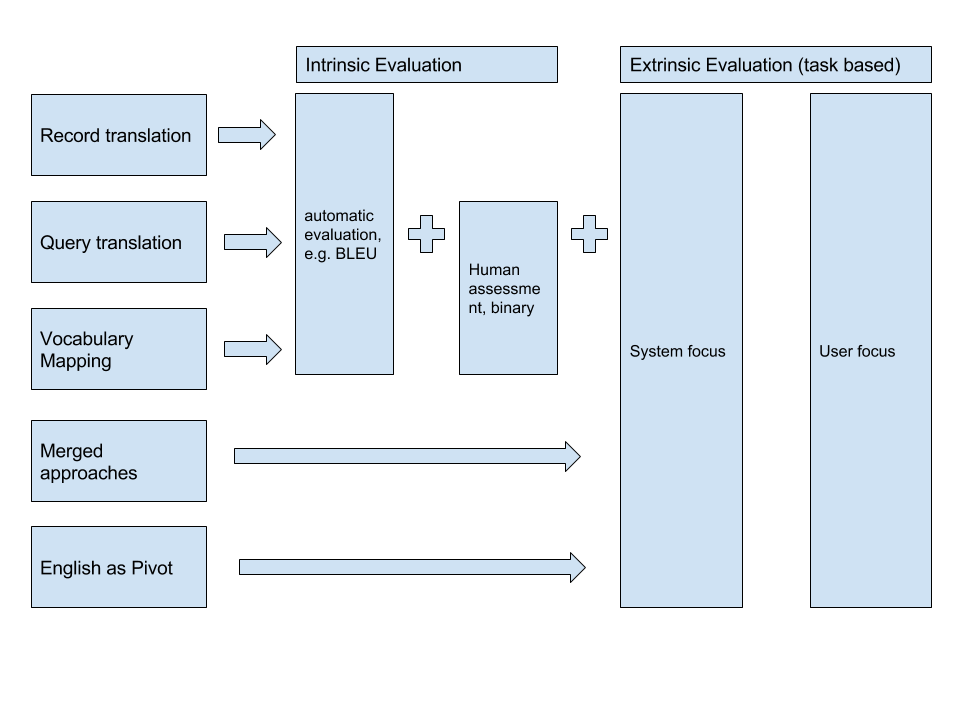
\includegraphics[width=0.8\textwidth]{./img/overview_evaluation.png}
	\caption{Evaluation plan for the different approaches tested in the project.}
	\label{fig1}
\end{figure}

First, the intrinsic value of each approach will be tested. For example, does the automatic record translation produce appropriate (i.e. correct) translations? This can be assessed automatically or be judged by a human. Once satisfactory results are obtained, we can move to the next step, the extrinsic evaluation. The extrinsic evaluation consists of different methods, which are either system- or user-focused.

In the system-focused extrinsic evaluation, we will look at the impact of the different translation approaches on retrieval performance, e.g. differences in result numbers and in the document sets retrieved. The system-focused evaluation will be performed using the set-up in Figure \ref{fig2}. Either the queries or the documents in the information retrieval system (here Solr) will change for the different translation approaches as described in the succeeding sections. Result lists from these evaluations will be compared to a baseline of result lists retrieved with untranslated queries and / or documents.

\begin{figure}[h]
	\centering
  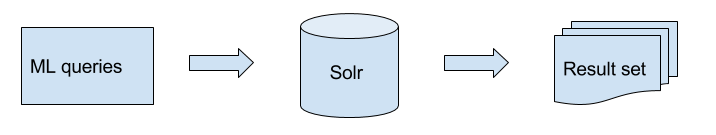
\includegraphics[width=0.8\textwidth]{./img/Info_sys.png}
	\caption{Set-up for the extrinsic evaluation approaches.}
	\label{fig2}
\end{figure}

The user-focused approach tries to incorporate the perspective of the users. This usually requires a judgment regarding the relevance of the retrieved documents. Additional user-focused evaluation could also take GUI changes with regard to multilingual features into account, shifting the evaluation approaches into user experience evaluations. 

The intrinsic evaluations will be done by DFKI/SU. Test corpora will be provided by Humboldt and ZPID. 

\subsection{Producing the Baselines for Extrinsic System-focused Evaluations}
\label{ss:baseline}
The basic set-up is shown in figure \ref{fig2}. In its essence, it will be used to produce the different baseline for the extrinsic system-focused evaluations. Since we want to exclude dynamic factors of collection or system updates (i.e. new relevant documents or new search features), which are independent from the translation, we will perform the evaluations on a stable (frozen) Solr instance with a stable collection of documents. A set of 50 queries manually translated into the four languages will be sent to the frozen Solr instance of PubPsych (see figure \ref{fig3}). The retrieved result lists will serve as a baseline for monolingual retrieval results. 

\begin{figure}[h]
	\centering
  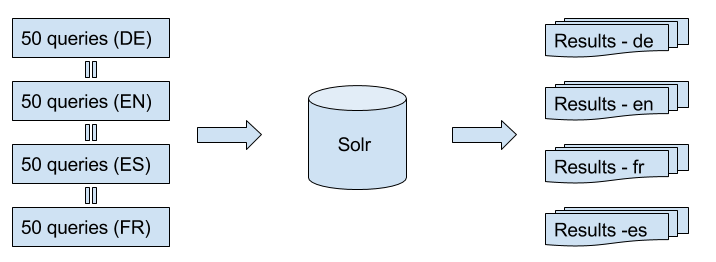
\includegraphics[width=0.8\textwidth]{./img/queries.png}
	\caption{Producing the baseline result sets.}
	\label{fig3}
\end{figure}

For each of the 200 queries, which are send to the frozen Solr version, the following information is saved:
\begin{itemize}
\item the results list
\item the number of documents retrieved
\item the ranked list of documents from the first result page
\end{itemize}

From the four different result lists of the aligned (i.e. parallel) queries in  English, French, German and Spanish, merged result lists can be created that contain all results of the four result lists. After removing the duplicates among the merged list, it can serve again as a baseline for multilingual retrieval.

\subsection{Summary of Experiments and used Corpora}

\begin{table}[h]
\resizebox{\textwidth}{!}{%
 \centering\textbf{}
\begin{tabular}[h]{p{2cm}p{3cm}p{3cm}p{3cm}p{3cm}}
    \toprule
    Approach & \multicolumn{2}{c}{Intrinsic Evaluation} & \multicolumn{2}{c}{Extrinsic Evaluation} \\ \hline 
    & Automatic & Human Judgement & System-focused & User-focused\\
    \midrule
	Record translation & 800 records in 4 languages & N/A &  50 queries in 4 languages & N/A \\
   
	Query translation & 250 queries in 4 languages & N/A & 50 queries in 4 languages& N/A \\
	Vocabulary Mapping & tbd & tbd & tbd & tbd\\

English as Pivot & same as for record and query translation& N/A & 250 queries in English &N/A\\
    Merged Approaches &  &\\
    \bottomrule
 \end{tabular}}
  \caption{Corpora used for the different experiments.}
 \label{tab:fields}
\end{table}

\section{Record Translation}

A record in PubPsych can have the fields aggregated in table \ref{tab:fields} with the respective candidates for MT. The fields \textit{key phrase} and \textit{additional descriptor} might contain relevant text for translation but are only provided by certain data sources or for a small fraction of records. Therefore, we decided to not include them in the machine translation.
\begin{table}[h]
 \centering\textbf{}
\begin{tabular}[h]{lcp{5.7cm}}
    \toprule
    Field name & Translation Candidate & Comments \\
    \midrule
	Title & X &\\
	Subtitle & X &\\
	Title translation &  &\\
	Author &  &\\
 	Affiliation &  &\\
	Country &  &\\
 	Source & & \\
	Year & & \\
	Journal title & & \\
	Media Type & & \\
	ISBN &  &\\
	ISSN & & \\
	Thesis title & X & Only present in source Psyndex\\
	Language & & language of publication, should be translated but not with MT \\
	Abstract & X &\\
	Additional abstract & X &\\
	Classification & X &\\
	Keyword/Controlled term & X & from controlled vocabularies\\
	Additional Descriptor &  &\\
	Age group & & \\
	Origin of Population & & \\
	Key phrase & & assigned freely by the cataloguer\\
	Controlled Method & & \\
	Document type & & \\
	Level of Evidence & & \\
	Segment &  &\\
    \bottomrule
 \end{tabular}
  \caption{Fields of a PubPsych record and the candidate fields for translation.}
 \label{tab:fields}
\end{table}

\subsection{Intrinsic Evaluation with Automatic Measurements}
Here, we use automatic measures, such as BLEU \cite{papineni_bleu:_2002}, to determine the quality of translation. Humboldt and ZPID provide an aligned corpus for this with \textbf{800} records that were manually translated from English into French, German, Spanish. 

\subsection{Intrinsic Evaluation with Human Judgment}
\underline{Note:} As the record translations are the means to improve cross-lingual retrieval, we will not evaluate translation with human judgements. If an intrinsic evaluation is required, it could look like this:
Annotators evaluate fluency and adequacy of the MT record. Fluency measures the translation based on its grammatical correctness, lack of spelling errors and natural language. It should be assessed by native speaker which can be monolingual. For the evaluation, a Likert-scale is often used \cite[Ch. 4]{chen_multilingual_2016}.

Accuracy measures how well the original meaning is transported in the translation. For this, bilingual annotators are needed. For both assessments, the inter-annotator agreement should be calculated.
Two states of MT output could be compared ranking the different translations \cite{Vilar:2007}.

\subsection{System-focused Extrinsic Evaluation}
Here, we will evaluate the record translation approaches using volume and result set differences in PubPsych by comparing the baseline result sets from the frozen Solr instance (see section \ref{ss:baseline}) with the result set retrieved with record translation. 
The query evaluation corpus consists of \textbf{50} queries aligned in English, French, German and Spanish. 

For the record translation evaluation, queries are fixed over the course of the project. The change is the translation of the record.\\

\underline{Methodology:}
\begin{itemize}
\item Each query (out of 50) is sent against the (untranslated) record collection and result sets are retrieved. These four result sets from the four languages are saved and used as the baseline resulting in 200 result lists.

\item After the record translation, the experiment is repeated with the same queries sent against the translated corpus (see Fig. \ref{fig4}). The evaluation compares the new result sets to the baseline result set. Each query should ideally retrieve more and different (better) documents than the baseline. 
\end{itemize}

\begin{figure}[h]
	\centering
  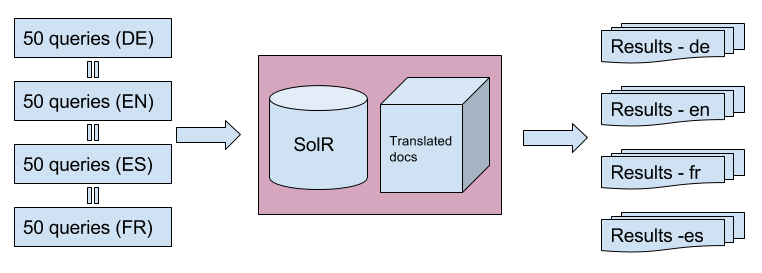
\includegraphics[width=0.8\textwidth]{./img/translated_docs.png}
	\caption{Retrieving result sets with translated records.}
	\label{fig4}
\end{figure}

\underline{Requirements:}
\begin{itemize}
\item Aligned query corpus of 50 queries in English, German, French, Spanish
\item Frozen Solr to produce baseline and new result sets
\item Translated PubPsych records (same as in frozen baseline corpus)
\end{itemize}

\underline{Evaluation Steps:}
\newline
We first compare result sets of same language queries usig the non-translated records vs the translated records. For example, the result set of a query in English (without record translation) is compared to the result set of a query in English (with record translation). 
\begin{itemize}
\item Compare results sets retrieved with the same languae query, we look at the size of the new result set (with record translation) compared to the baseline result set (without record translation).
\item Compare retrieved results to baseline, e.g. differences in found data sources.
\item Compare ranking of the first x results.
\end{itemize}

In a second step, we compare the merged results lists of each of the four aligned queries and compare it to the results list retrived with record translation. Here, the following measures are possible:

\begin{itemize}
\item Compare  the size of the new result set (with record translation) compared to the baseline result set (without record translation) retrieved from merging the results of four aligned queries.
\item Compare retrieved results to baseline, e.g. differences in found data sources.
\item Compare ranking of the first x results.
\end{itemize}

\underline{Example:}
\newline
Table \ref{tab:exquery} shows an example query “youth unemployment” aligned in the relevant languages. The result sets retrieved with no record translation can be compared to the result sets for each query when the records are translated (comparing the values in each column = 4 comparisons). Additonally, each result set retrieved with record translation can be compared to the merged list retrieved with no record translation (4 comparisons).
\begin{table}[h]
\resizebox{\textwidth}{!}{%
 \centering\textbf{}
\begin{tabular}[h]{llllll}
    \toprule
  &   "youth unemployment" & Jugendarbeitslosigkeit & "chômage des jeunes" & "desempleo juvenil" & merged list\\
    \midrule
  no record trans.  & 106     & 126     & 3  & 4 & 181\\
  with record transl.  & 183     & 180     & 185  & 185 \\
    \bottomrule
 \end{tabular}}
  \caption{Example of an aligned query and baseline number of retrieved documents.}
 \label{tab:exquery}
\end{table}

\subsection{User-focused Extrinsic Evaluation}
\label{ss:user_eval}
This evaluation is more focused on the user’s perception of relevance of the results. This could be done using A/B testing with result sets from the baseline shown and compared to the result lists of the adapted system. Ideally, the tests are designed to understand the impact of the record translation on user tasks such as determining the relevance of a document in relation to a query.

\underline{Note:} For all user-focused evaluations, we should leverage synergies. These evaluations are very costly and through thoughtful planning, we should minimize the effort here. One option is to decide for one user test which covers several scenarios.

\section{Query Translation}
\subsection{Intrinsic Evaluation with Automatic Measurement}

Here, we use automatic measures, such as BLEU, to determine the quality of translation. Humboldt and ZPID provides an aligned corpus for this with \textbf{250} queries translated in  English, French, German and Spanish. 

\subsection{Intrinsic Evaluation with Human Judgement}
This could be a binary judgement: correct or incorrect.
This could be also independent of an evaluation corpus, just sample some random queries and decide if the MT is correct or not. The feasibility of this approach depends on the complexity of the queries. Similar to the record translation, the intrinsic human evaluation is accompanied with increased effort. As the main concern is the impact on CLIR, we decided to forego this experiment. 

\subsection{System-focused Extrinsic Evaluation}
Figure \ref{fig:queriesMT} shows how the process could be done: the (frozen) Solr with the untranslated records is used and only the queries are translated. Each query is translated via MT into the respective other three languages (see table \ref{tab:queries}, the cells marked in green) resulting in 12 queries used for retrieval.

Three different evaluation steps are possible: 
\begin{itemize}
\item The results set retrieved in a monolingual search are compared to the one with query translations. For example, the result set of an English query ("youth unemployment") is compared to the one which were retrieved with the English query and the translation equivalents in German, French and Spanish ("youth unemployment" OR "Jugendarbeitslosigkeit" OR "chômage des jeunes" OR "desempleo juvenil"). This evaluation will assess the improvements of monolingual vs. multilingual  retrieval.
\item In table \ref{tab:queries}, each row contains 3 translations for queries (translation from the aligned corpus). The translated queries can be compared to the the manually translated queries. If queries are not identical, they are both sent to the Solr instance and results sets are compared. If the queries are the same translated by machine or by human, the results sets will be identical, too. This evaluation will indirectly assess the performance of the query translation MT. 
\item The last step would be to compare the merged list of each quadruple of queries which were manually translated to the one which was translated with MT.
\end{itemize}
 


\begin{figure}[h]
	\centering
  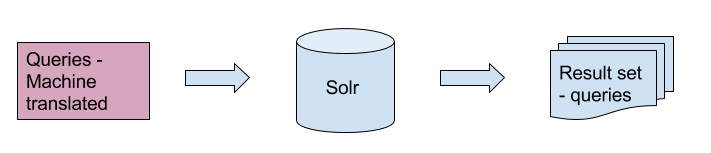
\includegraphics[width=0.8\textwidth]{./img/queriesMT.png}
	\caption{Evaluation approach for query translation.}
	\label{fig:queriesMT}
\end{figure}


\begin{table}[h]
 \centering\textbf{}
\begin{tabular}[h]{lllll}
    \toprule
    Aligned queries & From EN into & From DE into & From FR into & From ES into \\
    \midrule
	EN  &  -  & \cellcolor{green!25} EN  &  \cellcolor{green!25}EN  & \cellcolor{green!25}EN \\
	DE  & \cellcolor{green!25}DE  & -  & \cellcolor{green!25}DE  & \cellcolor{green!25}DE \\
	FR  & \cellcolor{green!25}FR  & \cellcolor{green!25}FR  & -  & \cellcolor{green!25}FR \\
	ES  & \cellcolor{green!25}ES  & \cellcolor{green!25}ES  & \cellcolor{green!25}ES  & - \\
    \bottomrule
 \end{tabular}
  \caption{MT translation of query sets into respective languages.}
 \label{tab:queries}
\end{table}

\subsection{User-focused Extrinsic Evaluation}
See Note under \ref{ss:user_eval}


\section{Vocabulary Mapping}
For the vocabulary mapping approaches, we will align the controlled vocabularies ideally in the four target languages. The vocabularies have to be identified. Existing mappings can be used for training and testing.

\subsection{Intrinsic Evaluation with Automatic Measurement}
Could be a precision-based measure based on already available mapped vocabulary terms, i.e. how many of the terms in one vocabulary are mapped to another one?

\subsection{Intrinsic Evaluation with Human Judgement}
This could be a binary judgement of the created mappings of a subset of the controlled vocabularies.

\subsection{System-focused Extrinsic Evaluation}

\begin{figure}
	\centering
  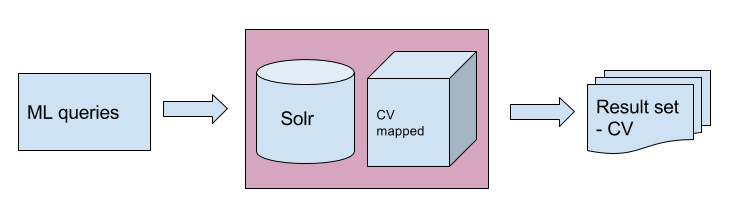
\includegraphics[width=0.8\textwidth]{./img/CV-Mapped.png}
	\caption{Evaluation approach for mapping of controlled vocabularies.}
	\label{figsystem}
\end{figure}

The methodology is very similar to the one we use for record translation, except that only the CV terms are "translated", i.e. mapped to the other languages (see figure \ref{figsystem}).


\subsection{User-focused Extrinsic Evaluation}
Testing the ranking for this might be very interesting. Overlap between queries and CV is crucial here. Also, see Note under \ref{ss:user_eval}.

\section{English as a Pivot Language}
\subsection{Intrinsic Evaluation with Automatic Measurement}
We can probably reuse the test we did for the record and query translations just using the English test sets. 
\subsection{Intrinsic Evaluation with Human Judgement}
We can probably reuse the test we did for the record and query translations just using the English test sets. 
\subsection{System-focused Extrinsic Evaluation}
We can probably reuse the test we did for the record and query translations just using the English test sets, see figure \ref{figpivot}. 


\begin{figure}
	\centering
  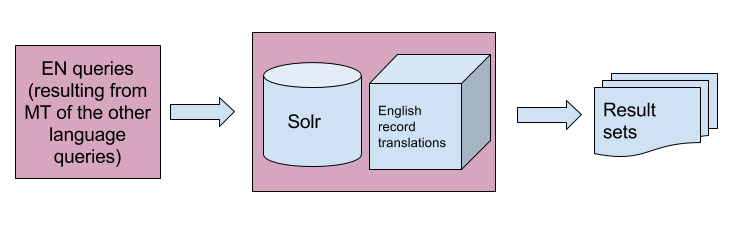
\includegraphics[width=0.8\textwidth]{./img/pivot_approach.png}
	\caption{Evaluation approaches for English as a pivot.}
	\label{figpivot}
\end{figure}

\subsection{User-focused Extrinsic Evaluation}

See note under \ref{ss:user_eval}.

\section{Merged Translation Approaches}
Here, we need to decide on the merged approaches to test. This could be, for example, the translation of all the records in the target languages + the mapping of controlled vocabularies. 

The evaluation set-up is then a combination of the set-up for the individual evaluation approaches above. For the user-focused extrinsic evaluation, we would look at different results sets. These could be merged to create synergies between the different evaluation steps.

\section{Comparing the Different Approaches}
So far, the different approaches were assessed comparing their performance to a system without any translation. We now need to define ways in which we compare the approaches against each other.
One approach is to juxtapose the different evaluation results and rank the approaches according to their performance. 

\subsection{User-Focused Extrinsic Evaluation}

%
% ---- Bibliography ----
%
\addcontentsline{toc}{section}{References}
\bibliographystyle{plain}
\bibliography{references}


\end{document}
